\chapter{The SAFE Network}
\label{ch:thesafenetwork}

\section{Decentralisation}

Decentralisation of data is the core benefit of the SAFE Network. As with many things in life, once someone has ownership or control of something they can either use that position of power for good purposes or for less desirable ones. The internet as it exists today is very fragile in this regard. When you upload a file to Dropbox\cite{dropbox} or OneDrive\cite{onedrive} that file exists solely on the servers that those organisations have control over. Once an organisation has data they can do with it what they please, acting within the bounds of overcomplicated privacy polices to manage user data. Not only does this incur the obvious privacy infringements but it can lead someone into the false sense of security that their data is safe. If someone managed to hack Dropbox or there was a catastrophic failure at the datacenter, a user has no assurances their data is safe. On a much larger scale companies like Amazon provide AWS\cite{amazon-aws}, an enterprise grade cloud-computing platform. If AWS were to fail, or be targeted, many of the worlds biggest websites would cease to function. This is because of the centralisation of resources. It is not necessarily an easy target, but it is a single identifiable piece of the equation that if removed, causes the whole thing to collapse.

Trust is at the core of decentralisation. Centralised control of resources requires trust in the facilitators of that resource. You have to trust that the resource is free of corruption and indeed trust that it won't be in the future. Companies readily change polices upon acquisition and managerial changes so this trust has to withhold over the course of time. Decentralised models of governance can be used to alleviate these problems. Through autonomous governance entities such as the SAFE Network can ensure equality to all participants. It achieves this through a system of `trust-less' cooperation between nodes. Vaults on the network do not inherently trust other vaults. Every action on the network must be reach a quorum before it is considered valid by the vaults. This autonomous self-governance is what decentralises the `trust' you must impart on the network to store data.

\subsection{Peer to Peer vs Client Server}

Centralisation of data and computing power is a natural consequence of the Client-Server architecture that has formed around the internet. It requires trust in the server you are interacting with. When you want to upload data that trust in the entity becomes a big consideration. The Client-Server architecture forces centralised governance, there is very much the idea of a central power and inequality between the participants in the network. A Peer to Peer (P2P) network encourages the decentralisation of power. In a P2P network participants are often of equal standing meaning no node in the network has more authority than any other node. Thus for a true decentralised network you have to have a P2P architecture to support it. 

The SAFE Network thus has to be built around the P2P architectural model. Nodes that comprise the SAFE Network are called \textit{vaults}. Vaults are responsible for both storing and serving data, they work together through an autonomous system of governance. Some vaults in the network have more authority than others,  these vaults are called \textit{elders}. To become an \textit{elder} a vault must first prove it is trustworthy and only after a quorum is reached between other vaults can it become an \textit{elder}. A vault of this status has more voting power than other vaults, using this power to reach agreements with other \textit{elders} and \textit{vaults} on all network decisions. This decentralised self-governance scheme is crucial to the autonomy and reliability of the network. Autonomy being a crucial pillar in the decentralisation of the network.

\begin{figure}
	\begin{center}
		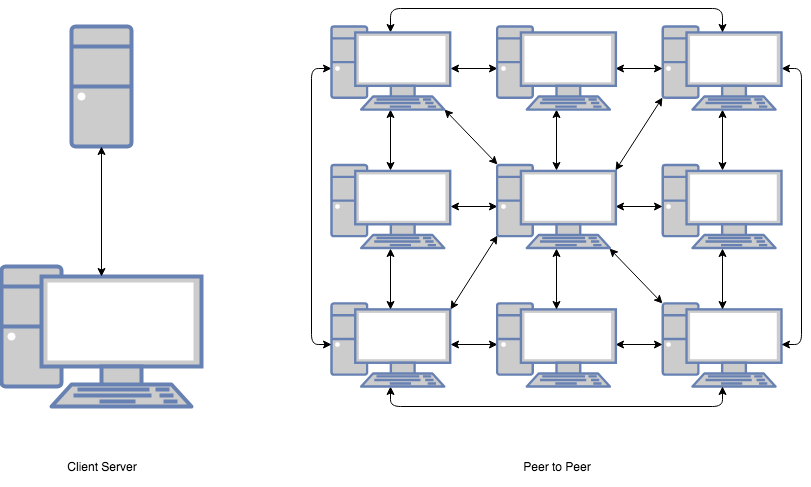
\includegraphics[width=\textwidth]{diagrams/client-server-vs-p2p}
		\caption{Client-Server vs Peer-to-Peer Network}
		\label{fig:client-server-peer2peer}
	\end{center}
\end{figure}

\subsection{BitTorrent}

The first stable version of the BitTorrent\cite{cohen2008bittorrent} protocol was released in 2001. Since then it has become one of the worlds most popular means of file sharing, accounting for \%3.5 of global internet traffic at the time of writing\cite{bittorrent-usage}. In a \textit{permission-less} environment users are allowed to freely share files with one another. As there is no centralised body controlling who has access to what data, the system has been widely used for the \textit{piracy} of copyrighted material. BitTorrent helps to solve many of the same challenges that the SAFE Network aims to. One of which is moving away from the traditional Client-Server architecture. In BitTorrent, peers form what is known as a 'swarm'. A 'swarm' is all clients that aim to download a a full copy of a piece of data. Data is broken down into discrete chunks, each with a unique hash that allows clients to uniquely identify each piece of the original file. A client in the swarm is known as a \textit{peer} when they don't hold a complete copy of the file. A client in the swarm is referred to as a \textit{seed} when they do hold a complete copy of the file. The 'resting state' of this network is when all clients in the swarm are \textit{seeds}. Nodes use P2P routing to send chunks of the file to other clients in the swarm that do not have it.

In BitTorrent there is no central 'server' to attack (disregarding a \textit{tracker}, there are \textit{tracker-less} solutions available). You can see the topology of a tracker based swarm in Figure \ref{fig:bittorrent-tracker}. Nodes can leave and rejoin the swarm whenever they want, as long as at least one node has a copy of a specific chunk then all clients in the swarm can spread the data and become \textit{seeders}. This level of data redundancy is a huge benefit to BitTorrent over a traditional client-server model of sharing files.

\begin{figure}
	\begin{center}
		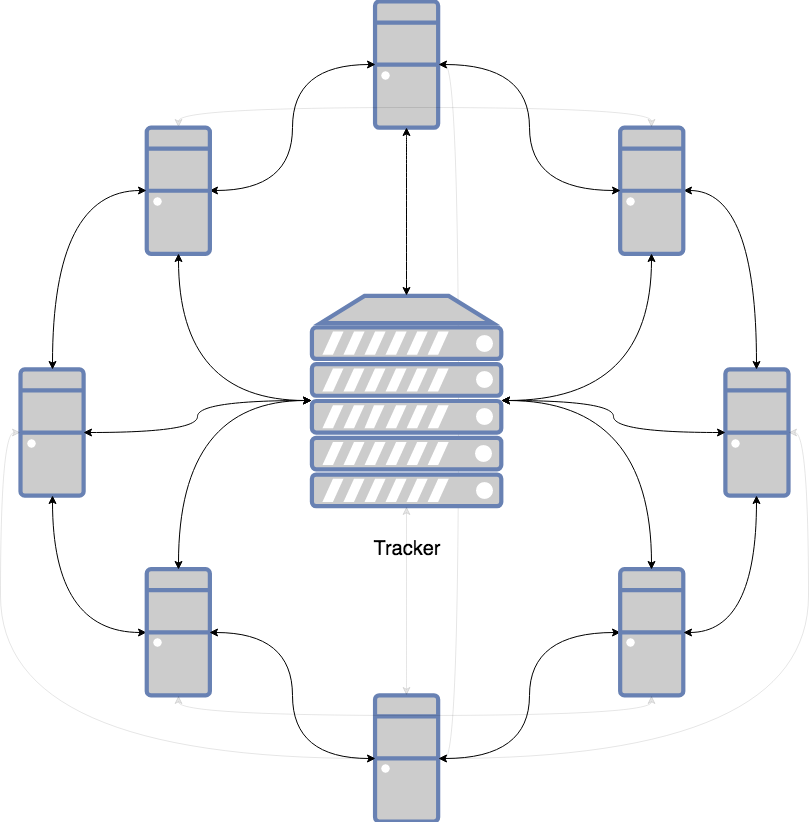
\includegraphics[scale=0.3]{diagrams/bittorrent}
		\caption{Topology of tracker based swarm in BitTorrent}
		\label{fig:bittorrent-tracker}
	\end{center}
\end{figure}

In the traditional model of file sharing, the owner of the server incurs great cost in the hosting of the file. They have to pay for the management, storage and the network costs of sharing that data. For large companies this is often a negligible cost that is not a prohibiting factor in hosting the data. For smaller organisations however (especially non-profits) this server cost can be a big problem. This is a primary reason why many Linux distributions so often provide BitTorrent links to download the operating system. By using BitTorrent they can offload the cost of sharing the file onto their users. This works on a `good-samaritan' basis where if you download a file you should aim to have your \textit{seed-ratio} hit at least 1 before leaving the swarm permanently (a nodes \textit{seed-ratio} is how much of the file they serve to other users against how much they themselves have downloaded from the swarm). For the vast majority of users this cost is negligible and can act as a 'good-will' gesture to help support projects.

Data transfer speeds are a major benefit of using BitTorrent and other P2P file sharing methods. When a node is acting as a \textit{peer}, their download speed is limited to the summation of the upload speeds of the nodes they are downloading from. This means that in a well established swarm that your file will download as fast as your internet connection will allow. The more users that join the swarm, the faster and more resilient to failures the network gets. This is juxtaposed to a client-server model wherein a single connection to the server must be shared by all nodes wishing to downloading the data. Thus download speeds are limited by the resources of that single server.

There is a crucial aspect of BitTorrent that means lots of organisations cannot make use it. The issue is that of control. Once shared, a file cannot be easily removed from the network. Thus not having ownership of data on the network makes it unsuitable for some applications. Notably this means that the distribution of copyrighted content across the network is very difficult, once shared you don't have any control over that data. Licenses change and legal implications mean that copyrighted material is often withdrawn from public meaning BitTorrent is unusable for such applications.

BitTorrent may solve many issues surrounding the distribution of files, but falls short of solving the decentralisation of the internet as a whole. The main limitation being that data on BitTorrent is not mutable. Once a file has been spread to a \textit{swarm} it is an immutable entity that cannot be changed. This means it is extremely challenging to use BitTorrent for dynamic content such as websites. Immutability is a big drawback depending on the use case, thus the option to support both Mutable and Immutable data is beneficial. The other attributing factor is that data only exists inside \textit{swarms}, you cannot interact with data without first joining the relevant swarm. So the discoverability of data is an issue. A given node within the network can't work out how to retrieve a chunk of data that is not located in the swarms it belongs to. These are all points that the SAFE Network offers solutions to.

\section{Serverless Architecture}

The idea behind a serverless architecture is to move as much computation/functionality to the client as possible. As time passes, the computational power of user workstations gets faster and faster. This computational power goes wasted for the most part. When you browse the internet, interact with Facebook for instance, your computer actually does very little in terms of processing the information you are seeing. Facebook serves to your browser a thin-client which can then make requests to Facebook for the data that is needed. Thus there is untapped potential on client side to perform more work locally instead of doing it server side. 

There are drawbacks in offloading work to the client. The first issue, especially with websites like Facebook, is privacy. When Facebook processes the data on their servers, they can assure that only data you are allowed to view is sent to your client. If this data was processed locally it would introduce new challenges in data protection and security. Another drawback is that of mobile devices. On laptops, smartphones, tablets and IoT devices power consumption is a major factor. Thus by using the traditional client-sever model you can offload the electricity expensive computation to the server and reduce power consumption on the device. This is in combination with reducing bandwidth to the client, which for mobile devices is a crucial factor in battery life. This means that when using the serverless architectural model in battery powered devices power consumption and network traffic must be minimised as much as possible. Not an easy task when large amounts of data need to be processed for rich and interactive content.

Vaults serve a similar purpose to \textit{peers} in BitTorrent. Note that they do not serve a similar function to \textit{seeds}, the network aims to never keep a complete copy of a single file in a single vault. The SAFE Network in this capacity can then serve a similar purpose to BitTorrent. Additionally what the SAFE Network has is the ability to route requests throughout the entire network. All \textit{vaults} in the network have the knowledge required to find any chunk of data. This is different to BitTorrent because it can only find a chunk of data within the swarms it knows about. As this dynamic routing exists, the SAFE Network has a form of DNS that can be used. Another major difference is the SAFE Network is capable of mutable data. This means that the SAFE Network is fully capable of supporting dynamic websites, forums, email and other such applications. You can open a browser that is capable of connectivity with the SAFE Network and browse the \textit{internet} just as you would normally.

From the clients perspective, a vault only serves and stores data. No processing of the data can be performed on the vault. Thus SAFE Network applications must process all the data locally and only use the network as its storage 'back-bone'. Thus the \textit{Serverless Architecture} model is a good fit for the SAFE Network. This method of building websites and applications has been around for a long time. With the advent of JavaScript and other such technologies, it was possible to run code locally through the browser without needing the server to do any processing. A good example is online mini-games, the code runs locally and there is no processing required on the server. The JavaScript/Flash/Java/... code is served to your client and the processing is performed locally. Another example of this are online \textit{office suites}, they are very powerful programs that can be ran through the browser. They depend heavily on the processing power of the client to provide an experience similar to that of a desktop application.

The SAFE Network forces the \textit{serverless architecture} architecture to be used unless you merely use the SAFE Network as a component in your stack. This introduces challenges in how you build and design applications. As you no longer have servers, you don't need to consider how your apps data will be served. This means that you can save time and cost in developing the 'back-end' to your software. Instead of designing websites and applications the \textit{traditional} way, you develop them like you would a \textit{fat-client}. Websites will become heavier, requiring more care and optimisations. Messy and slow JS is abundant in the internet today, mostly due to the abundance of computing power that exists. This hap-hazard way of coding cannot exist for \textit{serverless architecture} websites or applications. As discussed previously, battery life is an important consideration when offloading work to the client. This means that applications/websites that follow the serverless architectural model must be well optimised for power consumption. A new technology that is emerging that can help aid this is WebAssembly.

\subsection{Web Assembly}

Web Assembly is an assembly-like language that you can compile C, C++, Rust, etc, to and then run inside web browsers. It allows you to write code in high-level languages (that aren't interpreted like JS) and then serve it to users such that the code runs with \textit{near native} performance. This has big implications for the internet as a whole, not just the SAFE Network. A technology like Web Assembly could therefore be extremely useful when building websites that use the \textit{serverless architecture} model. A big strength of Web Assembly is in the processing of data. You can more easily write high performance code to process data in languages like C than you can in JS. Since the SAFE Network serves raw data to the client, the use of Web Assembly to process it could be a huge aid in increasing performance on lower power devices.

\subsection{Serverless Fat Clients}

A \textit{Fat Client} is a computer (application) that can perform operations and tasks without relying on a central \textit{server}. A Fat Client may still need to make periodic connections to a server but the vast majority of its functionality can be performed without \textit{chatter} with the server. The concept of a Fat Client is juxtaposed to that of a Thin Client. A Thin Client is a lightweight computer/application that relies heavily on a server to have any sort of utility. It can perform some tasks locally but most are processed on the server before being sent to the client. Although not all Fat Clients follow the \textit{serverless architectural} model, applications that are designed to be \textit{serverless} are inherently Fat Clients. Hence because of the points mentioned previously, the SAFE Network encourages (almost requires) the Fat Client style of architecture to be used for software development. As Web Technologies mature they become more and more suitable for the development of fat clients. Instead of having to download desktop applications to your device, new technologies allow rich \textit{serverless fat client} applications to be built and delivered through the web. This prevents users from having to change the way they browse the internet. If delivering \textit{serverless fat client} applications through the web was not possible, users would be required to change to a model where they would have to download an app for Facebook, Twitter, YouTube etc. Hence I view the advent of new Web Technologies, such as Web Assembly, to be an enabler in the success of the SAFE Network.

\section{Ownership of Data}

Accessing the SAFE Network is \textit{permission-less}. What this means is that users don't need to go to a central body that controls the network to ask for (register) an account. A user simply connects to the network and is allowed to create one. All users of the network are equal, there is no concept of `admin' accounts. When a user uploads a piece of data to the network, it can either be `public' data or encrypted data. Note that all data stored by \textit{vaults} is encrypted, if the data is `public' then it means that the decryption key is publicly available so anyone can access the data. Vaults are still unable to determine the contents of the encrypted chunks they are storing.

In decentralised data storage networks tying ownership to real-world identities is difficult. In many cases there is simply no means to facilitate this. Ownership of data is one feature that the SAFE network provides as apposed to a system like BitTorrent. In BitTorrent, its not possible to uniquely identify the owner of a piece of data. If a user starts sharing data they might be the theoretical `owner' but owing to the design of the protocol they have no ability to control the data. All users in a BitTorrent \textit{swarm} have equal rights to data. In the SAFE Network, the ownership of data is more clearly defined. When data is uploaded it is split up into chunks and distributed across different vaults. Owing to the design of the SAFE Network that data has an identifiable owner, the account that originally uploaded it to the network. They can do with it what they wish, including deleting the data permanently. This contrasts with BitTorrent greatly wherein data cannot simply be deleted. To delete data in the BitTorrent network you would have to explicitly ask all nodes to delete the file, they have no obligation to do so.

Data that has been written to the SAFE Network is \textit{immutable} without the credentials of the account that uploaded it. This is beneficial to users as it means they have the assurance that they own and control their own data, nobody else can edit or tamper with it. This does however incur issues surrounding the distribution of illicit and copyrighted content. A scenario I can envision is users treating accounts as `disposable'. One could imagine someone uploading the latest Hollywood blockbuster and then erasing the account credentials used to upload that file. Once lost, it is impossible to delete the data from the network. A solution to this could be through the use of a \textit{master-key} to the network. This would be a decryption key that would allow complete access to all data on the network. Such a key would be beneficial in removing illicit content but completely invalidates the principles of the SAFE Network. This issue of control has made a huge impact upon BitTorrent, numerous court cases and law suits have been issued since its inception down to its use for illicit content sharing. This is a situation of "you can't have your cake and eat it too". It is impossible to ensure complete security of user data and then undermine that with the ability of a central body to tamper with it. At the end of the day the SAFE Network is a tool. Like any other tool (BitTorrent) users will do with it what they please. The mitigation against illegal use of the tool should not impact on those who follow the law.

\section{Alternative Business Models}

Like any new technology, the SAFE Network opens up many opportunities that didn't exist before. In SAFE Network nomenclature, \textit{vaults} farm data. The safe and reliable storage (farming) of data is rewarded with \textit{Safecoin} which is a cryptocurrency built into the SAFE Network. One could envision an application that instead of charing users for access, allows them to become a vault that generates Safecoin. This Safecoin could then be sent back to the creators of the program and hence financially compensates them for the usage of their application. One consideration of this approach however is that vaults don't get to choose what data they store, that is an integral part of the architecture of the SAFE Network. By following this financial model then it would be for the 'good of the whole', increasing the utility of the entire network and not just for one application.

This model could be used to better make use of a consumers resources. When a user sits and watches Netflix on an entertainment system, there is very little strain on the resources of the device. In the case of a games console, literally teraflops of processing power, advanced networking and storage facilities are going unused. Potential financial models can try to \textit{exploit} this untapped power to the benefit of both the user and the provider of the application. One possibility facilitated by the SAFE Network is \textit{farming} \textit{Safecoin}. Not only does this increase the utility of the SAFE Network but provides users with an entirely new way to pay for content. Offering the resources they have in exchange for access to services.

\section{Architecture of the SAFE Network}

The SAFE Network is still very much in active development. At the time of writing, the SAFE Network is currently on its second alpha revision (Alpha 2) out of a planned four. The network is thus still very much subject to rapid changes. Chapter \ref{ch:architecture} explains the architecture of the SAFE Network at the time of writing.